\section{New Public Transport Technologies}
\label{sec:newtech}
In this paragraph, as previously stated, we are going to analyze the public transport future requirements that, in term of technologies, are becoming increasingly stringent. In order to be competitive on the bus market, the vehicles have to be equipped with a lot more technologies than nowadays. The technologies are needed since the world now is demanding more an more data and insight on every activity, not only from a general and distant point of view, but from a direct, punctual and real-time view. Nowadays Public Transport in Italy, and buses in particular, are often equipped with close to nothing technologies that can improve the service; as we have seen in the previous chapters, Arriva buses are quite old as well as the systems used to collect the data: all the spreadsheets concerning the service, control management, balance sheets were clearly written by hand.

Public Transport technology innovation is not just the systems that can be installed onboard, such as the AVL or APC, but also all the world that revolve around them, from the service’s planning and management to the data gatherings and costumer feedbacks. All the innovative technology can be divided in two big groups: the systems that are installed directly on the buses, and the systems that operate remotely, off the buses.


\subsection{Technologies installed on bus}
\label{subsec:techonbus}
The purpose of on – bus technology is mainly service monitoring and data gathering for demand analysis and offer adjustments, those type of system have become particularly relevant in the, very recent, Covid–19 period where it was particularly relevant analyze and report the mobility evolution to prospect near future scenarios and assess the effectiveness of adopted actions.

\begin{figure}[h!]
    \centering
    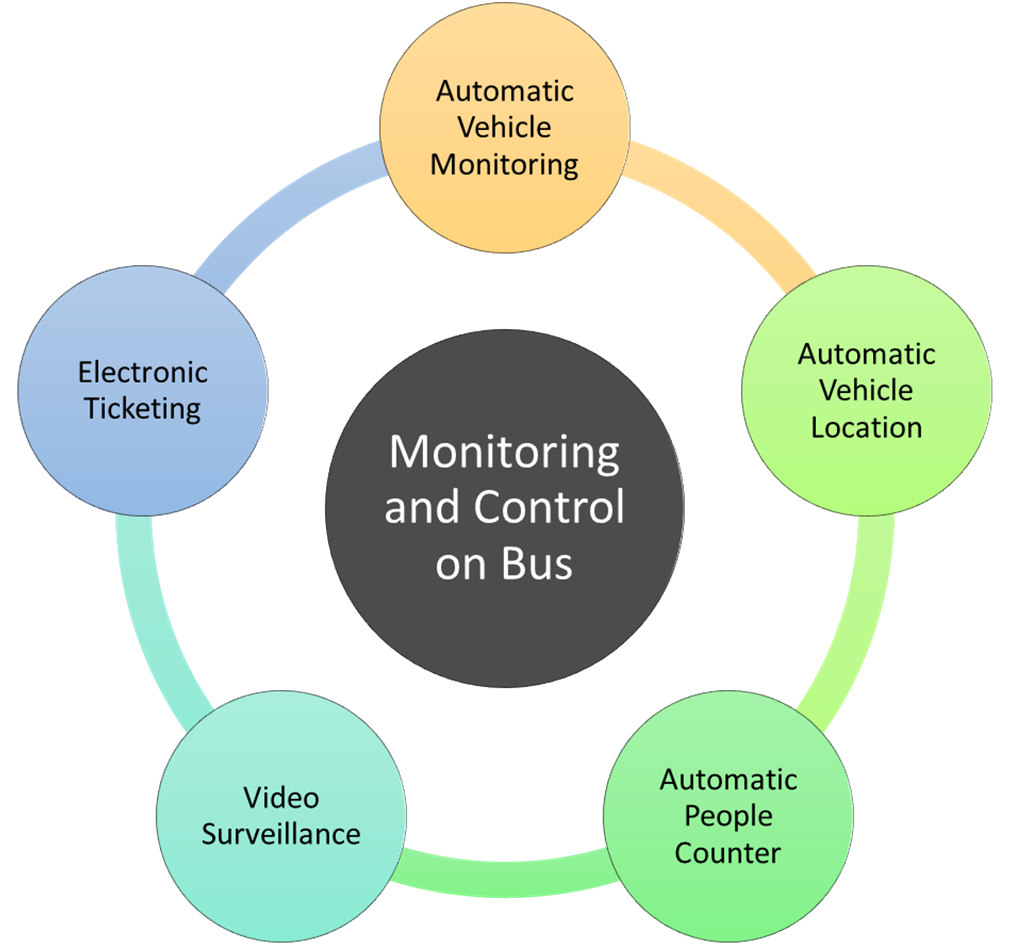
\includegraphics[width=0.6\textwidth]{Images/New Technologies/immagine intro Tech On.png}
    \caption{Technology Installed on Bus}
    \label{fig:onbus}
\end{figure}

\paragraph{AVM and AVL}
Automated Vehicle Monitoring is a technology based on localization through GPS, monitoring and recording different topics related to moving vehicles, such as position, speed, diagnostic of mechanical components and so on. Automated Vehicle Location is more focused on the GPS position on the vehicle but if GPS signals are poor, AVL can use different technologies to determine actual location information, such as dead reckoning, which takes a previously determined position, and then incorporates estimations of speed, heading direction, and course over elapsed time. 

The buses, based on the GPS signal that the satellite sends, calculate their position a certain amount of seconds. This information, together with other data, is sent to the operator in the operation centre which operate in real-time the data and sends them to the costumer information management systems. Those data are also stored in order to make them available to the procuring entity for service reporting.

This type of technology allow the PTO to increase the security level and control in case of disruptive events, being able to handle and analyze big amount of data to assess a quick result or motivation.

Those technologies can be used to compute some interesting KPIs, tacking the status of the service, advances and delays, vehicle tracking, service adjustments in case of disruptive events. Also, from a graphical point of view the real-time situation can be displayed really well and it can be used widely in a dashboard.
\begin{figure}[H]
    \centering
    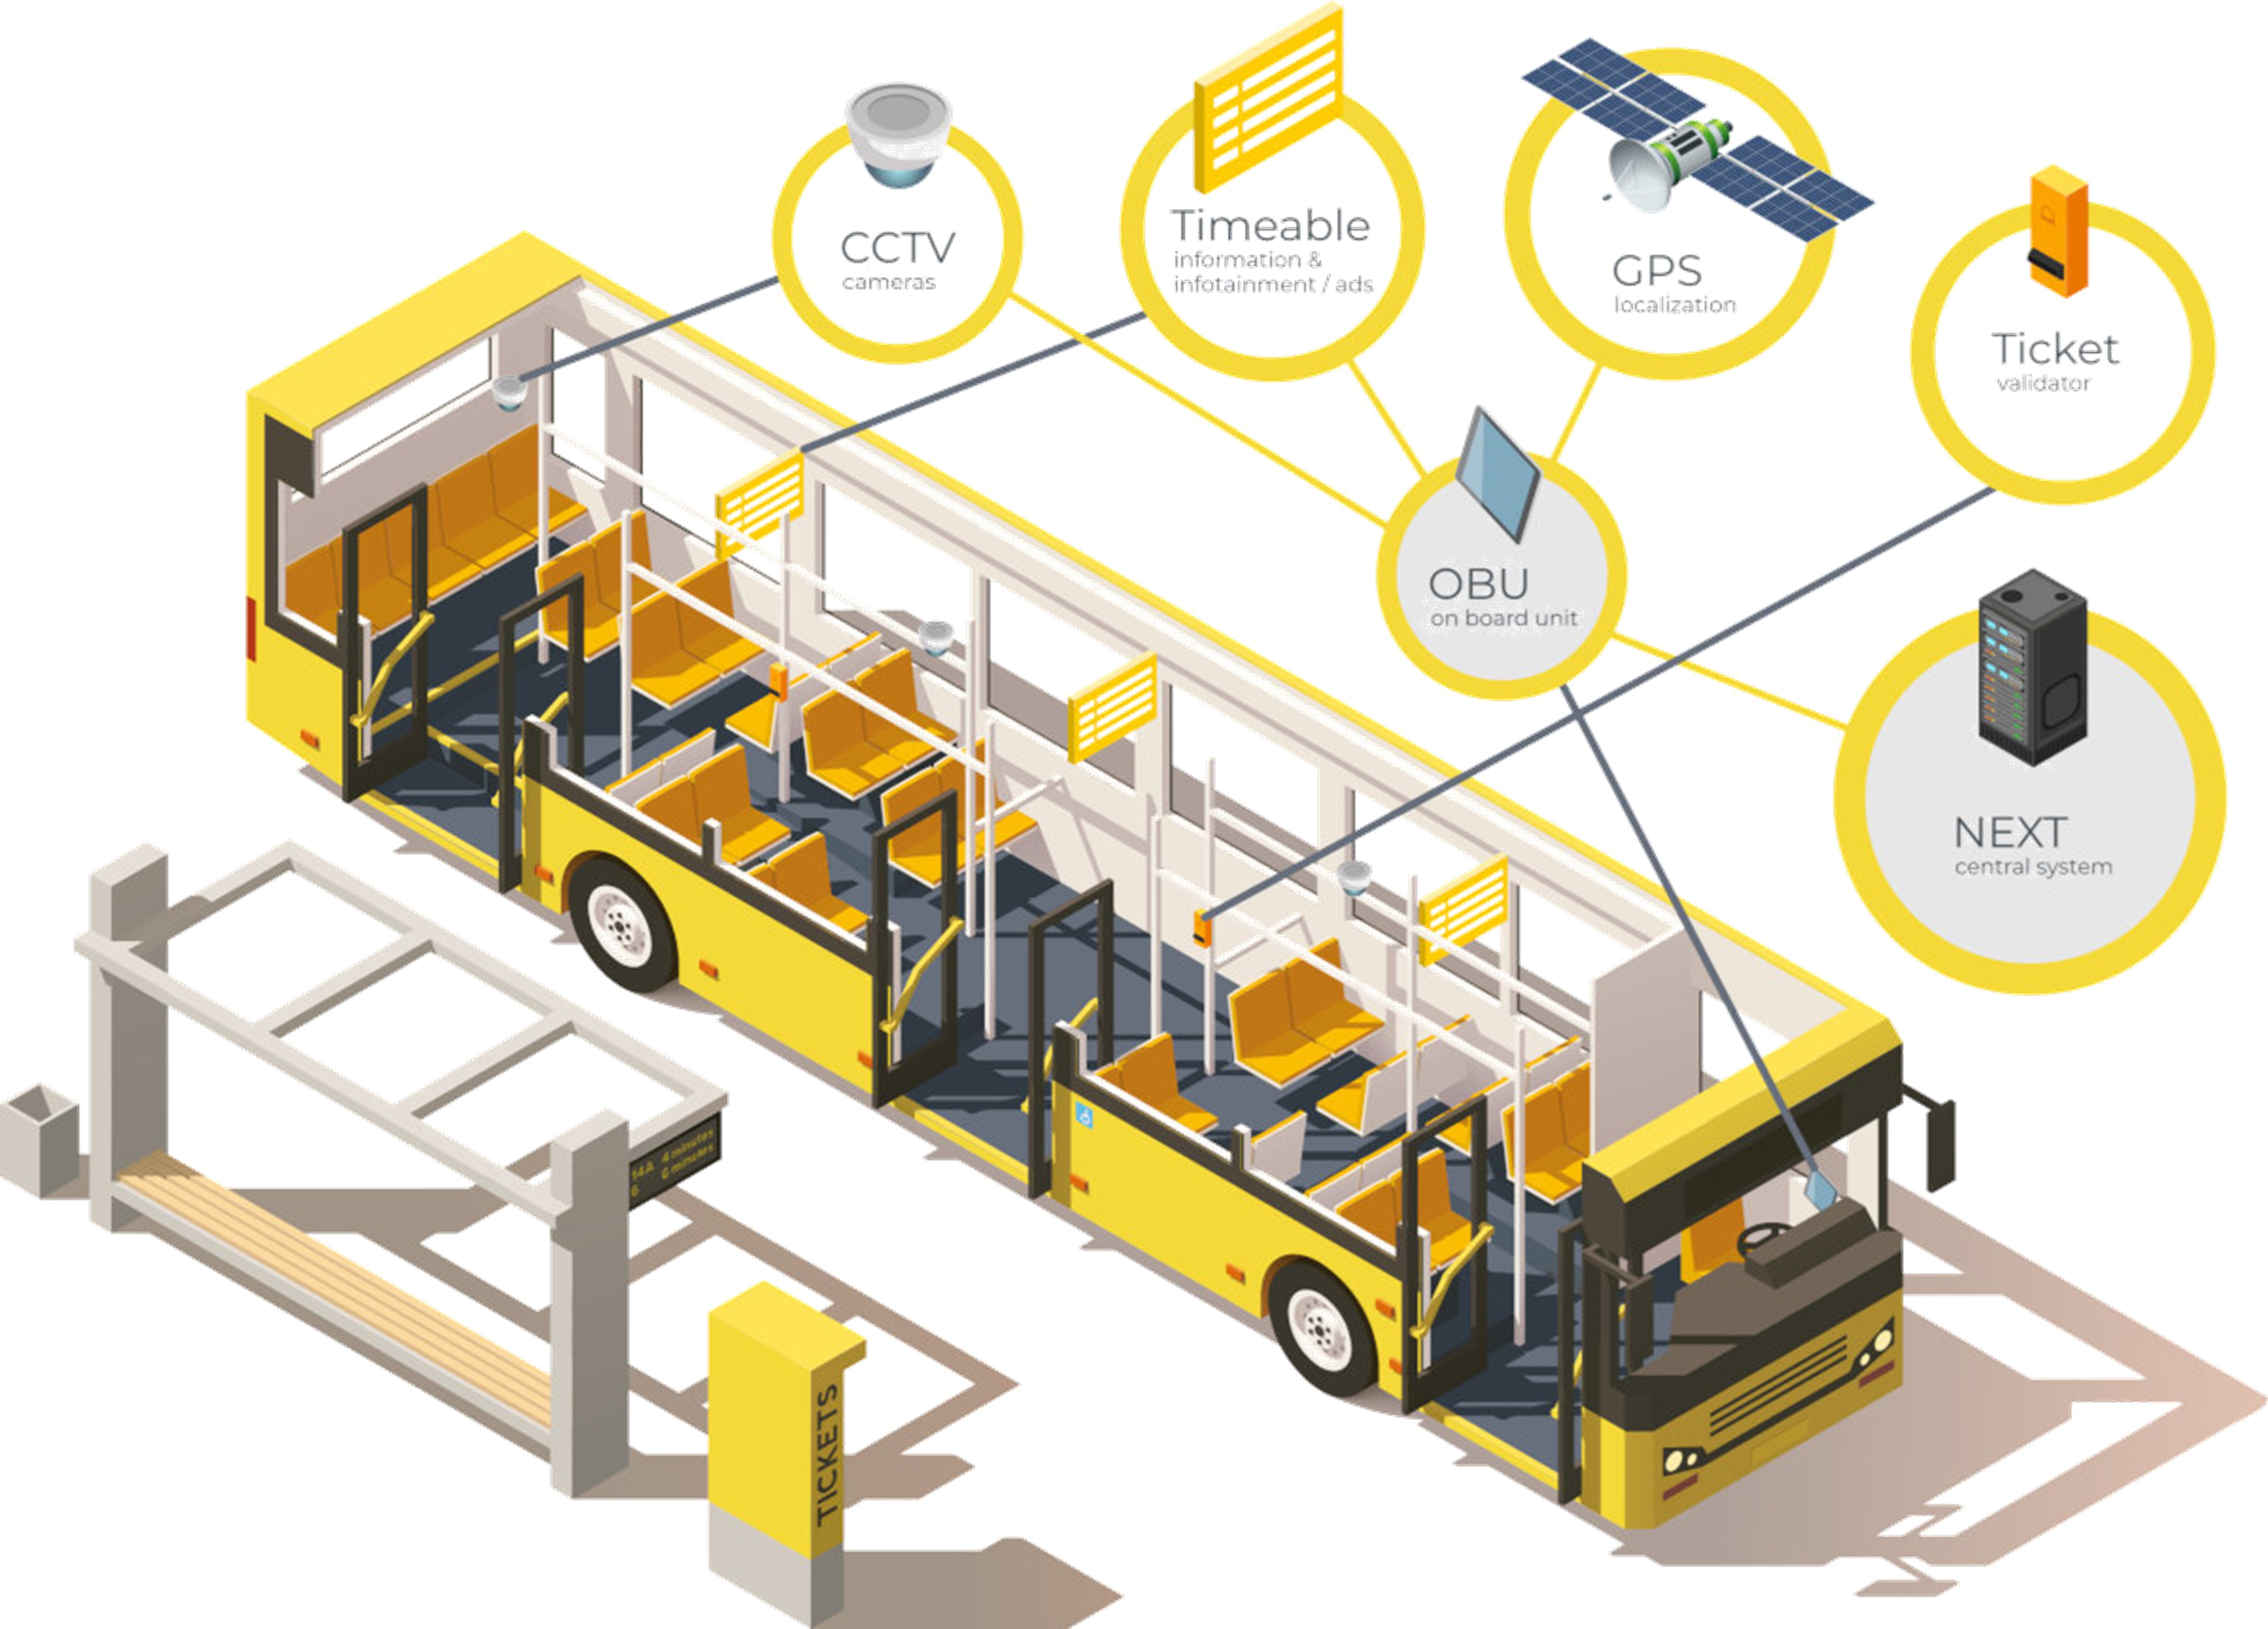
\includegraphics[width=0.7\textwidth]{Images/New Technologies/AVMeAVL.jpg}
    \caption{AVM and AVL}
    \label{fig:avmavl}
\end{figure}

\paragraph{Automatic People Counter}
People counters are electronic sensors that count people as they walk into an entrance. There are various methods for those systems to count people. Those can be classified into contact-type counters, sensors implemented system, and vision-based system using a camera. Contact-type counters are mechanical counters which need human contact such as turnstiles and mat-type foot switches that can obstruct the path. 

However, this type of counter only applicable for minimal people counting and it is not suitable for massive number of people, such as a high flow of people boarding or getting off the bus. Other technologies used in people counter are Pyroelectric Infrared (PIR) sensors, ultrasonic sound distance sensor and thermal sensor. PIR sensor counts people when they pass through the area of observation which is mounted with a pair of IR transceiver. Thermal sensors are only able to observe the crowd density without counting them accurately. 

\begin{figure}[h!]
    \centering
    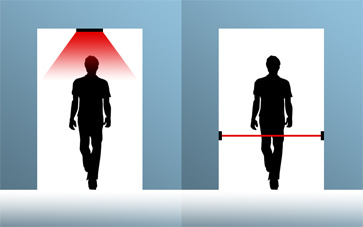
\includegraphics[width=0.5\textwidth]{Images/New Technologies/APC.jpg}
    \caption{Automatic People Counter}
    \label{fig:APC}
\end{figure}

People counting technologies can be used for many purposes: assessing that is impossible to have them on all the lines of the consortium, it is possible to use a data analysis on routes that do not have APC to build a model to estimate the level of service onboard on all routes. The load factor information is very useful to consult on a real-time dashboard, creating a trend of the number of people on board; in this way it is also possible to study the performance of the stops, as well as the lines, creating a set of KPIs that can function both as real-time  indicators and for decision-making at a future planning level.

\paragraph{Video–surveillance }
Video-surveillance is a technology that is extremely helpful for public transport management; cameras can be installed in three main positions: outdoor cameras, to monitor the surrounding scene and in particular the blind spots, indoor cameras, to monitor bus passengers, and driver cameras, to monitor the driver behaviour. All those images can be provided to the driver with clear images referring to these areas, which can then be displayed on special monitors to be installed on the driver's dashboard. 

With the new telecommunication technologies, like 4G and 5G, it can be performed a sort of edge computing through the help of video analysis with AI systems; these methods can lead to fast and responsive actions or adjustment that the drivers, or the employees in remote, can do. Artificial Intelligence algorithms can detect some risk factors for what concern the ride’s safety, such as tiredness, distraction, or irregular behaviour of the driver.

\begin{figure}[h!]
    \centering
    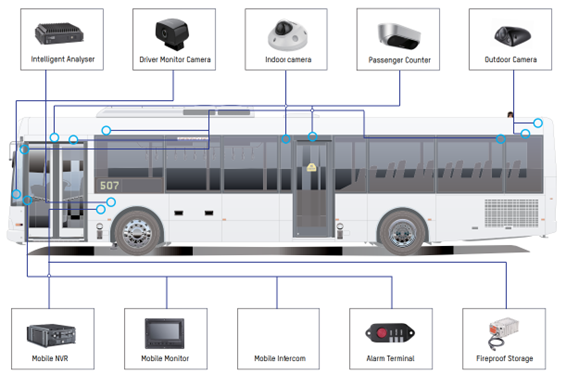
\includegraphics[width=0.8\textwidth]{Images/New Technologies/VIDEOSURV.PNG}
    \caption{Video–surveillance}
    \label{fig:vs}
\end{figure}


\paragraph{Electronic ticketing systems}
The electronic ticketing system is not a proper technology installed just on buses, but the validation and control parts are managed largely on the bus. The system is composed by the validators and the On-Board Computer, which are installed directly on the buses, and by a central Control Center where all the data collection, management and distribution of incomes and emission or recharge of smart cards takes place.

\begin{figure}[h!]
    \centering
    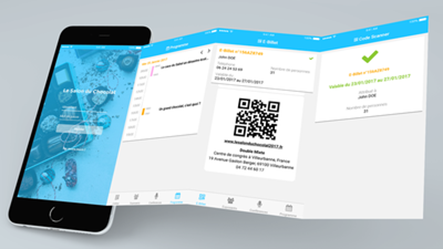
\includegraphics[width=0.6\textwidth]{Images/New Technologies/ELECTRONIC TICKET.png}
    \caption{Electronic ticketing systems}
    \label{fig:ets}
\end{figure}

One of the trending topics on the whole ticketing system is the type of support used: the support is the connection between costumers and PTO, which means that more information the support can bring to the PTO the better it is. In recent times there has been a rapid evolution of the support type, starting from basic paper, passing through magnetic, smart-cards and lastly mobile tickets. With Near-Field Communication (NFC) technology, the fares are redeemed without contact and completely remove the need to handle any physical cash or fares, and even limit the interaction needed with the driver. An additional motivation is that it is been found that physical money can carry the virus (in particular Covid-19) for up to three days, and by bypassing the need to purchase paper tickets and validate them, mobile ticketing can help reduce the transmission of the virus between riders and staff. An incredible by-product of integrating this technology is also the impact it has on the environment, as physical tickets no longer need to be created.

Keeping the user in mind, public transit technology is moving toward creating a more personalized ridership experience. A shift in this space is Account-Based Automatic Fare Collection. Through this system, all travel history, documents, and account information for riders is gathered in a customized dashboard.

With this technology, passengers can identify and participate with every available public service that is enabled for Account-based fare collection, making it far easier to use different modes of transportation, and save specific routes or journeys for use later. This also removes the hassle of having to manage multiple user accounts, payment methods, and receipt/billing information.

\subsection{Technologies installed off bus}
\label{subsec:techoffbus}
In addition to technologies directly installed on buses, there are some systems that play a center role in the world of public transport innovation, even not being directly on the public transport vehicle. Those type of technologies are aimed more at the network part of the service: we are talking about all the secondary, or subsidiary, technology that are vastly growing in the world, that together form the infamous Internet of Things. 
The general concept is that public transportation is affected by countless variables and not only by the ones directly connected to it, such as the costumers, the bus health, the drivers and so on, for example: the weather is clearly a source of data in correlation, but more importantly in causation, with the transportation system, if a day there is a particularly heavy rain, people tend to use more the private vehicle, using less the bus or in general the public transportation, this is due to the fact that often using PT means waiting outside under the rain. This situation have a great impact on the PTO systems, in fact bus tend to be less populated, so all the KPIs related to the number of costumers onboard are affected, as well as the travel time since, as said before, there are more private vehicles on the road than in a normal day; travel time therefore will be higher than usual and more delays, all of this affect the KPIs related to the commercial speed, travel time, delays per day and so on…
This big example is made to understand that the more data of different types are gathered daily, the more precise the analysis that a PTO can assess. In this new era of technology, especially now with the faster growing 5G, it is very important to take advantage of them, exploiting all of their potentialities.
The potential of digital applications and solutions for public transit is endless. Sensing devices and IoT technology are becoming more robust and low-cost, providing useful data for municipalities, fleet managers and even riders. For example, in Sweden a recent study used wireless sensors on city buses to monitor real-time air pollution. The sensors gave more accurate data on highly polluted urban areas, which led to better-informed city planning decisions and air quality improvement efforts. 
Telematics technology is also becoming a way to provide transportation fleet managers with real-time data to help identify and address things like temperature control, fuel levels, optimal driving routes, operating efficiencies and more. Predictive analytics allows for quick maintenance and better energy management, which is critical to addressing environmental impact.
Other important aspects of this topic are the actions that the PTA can take directly, for example, with the spread of smart cities, the necessary information and communication infrastructure lends itself well to intelligent traffic management systems. These systems allow centralised traffic control, enabling transit authorities to intelligently manage traffic lights, cameras, emergency routes and public transport routes.

Urban transit systems are also looking into how to incorporate rapid transit into existing systems. While this term most often refers to rapid transit trains or hyperloop systems, this can also refer to rapid transit buses, which have dedicated traffic lanes and priority at intersections; something that smart traffic management can help manage.


\subsection{New KPIs possibilities}
\label{subsec:newpossibilities}
As we have understood in the previous paragraphs, frequency in data–gathering is a key factor. Looking at the data provided to us is almost surprising that a company like Arriva, and all the consortium in general, has such a lack of detail in the available data. The dashboard built in the previous chapter has a potential, clearly limited by the frequency and the quality of what’s inside.

But why a higher frequency data – gathering is the base answer to most of the problems? Gathering more data more frequently means that it becomes much easier to understand trends, seasonalities, or particular micro – behavior that a monthly, or in some cases even yearly frequency cannot pick. In particular, algorithms like regression, classification, clustering, anomaly detection, and many others, work so much better with large quantities of data, and therefore understanding what they have to tell us is far easier.

Another strong motivation for why is essential to have data gathered more frequently is the possibility of expansion of the analysis that can be done: looking at a more detailed time span is useful to build a model on different types of time centered analysis, such as workdays vs. weekdays, peak hour vs. off-peak hours. The possibilities of Arriva, as now, are to compute KPIs based on the company trend of the month or year, which can hide an enormous quantity of information; having daily, hourly, or even more precise data, allows the analysts, and us, to build a dashboard with better KPIs.

\paragraph{Dynamic KPIs}
Other than more precise KPIs, gathering all those types of data can mean also being able to compute different \textit{types} of KPIs: we are used to looking at dashboards with basic cardinal numbers, which by definition are static and provide agglomerative information on the subject, such as a mean, a median, maximum or minimum and so on. 
Introducing the use of \textbf{Dynamic KPIs} opens up a new dimension in the data – plane in which the analyst can look and assess more types of conclusions. The Dynamic KPI is a particular way to view a result where the user can look directly at the trend, in real-time of the data, but let’s make an example.
If we want to analyze the number of passengers on – board on a specific ride, until now the KPIs were all built as a mean number of the occupation on – board, representing the average number of passengers on that ride. But this information, which is still useful, don’t get us wrong, is not able to tell the users how the flow of passengers distributes among the stops of the ride. Using a dynamic KPIs that shows both the people loaded and unloaded at every stop, we can see in the data more information, such as a particular section in the run where there are very few people on – board, and if it is behavior repeated in time, this information is useful to assess some conclusion, such as remove some stops, add new ones and many more.

\begin{figure}[t]
    \centering
    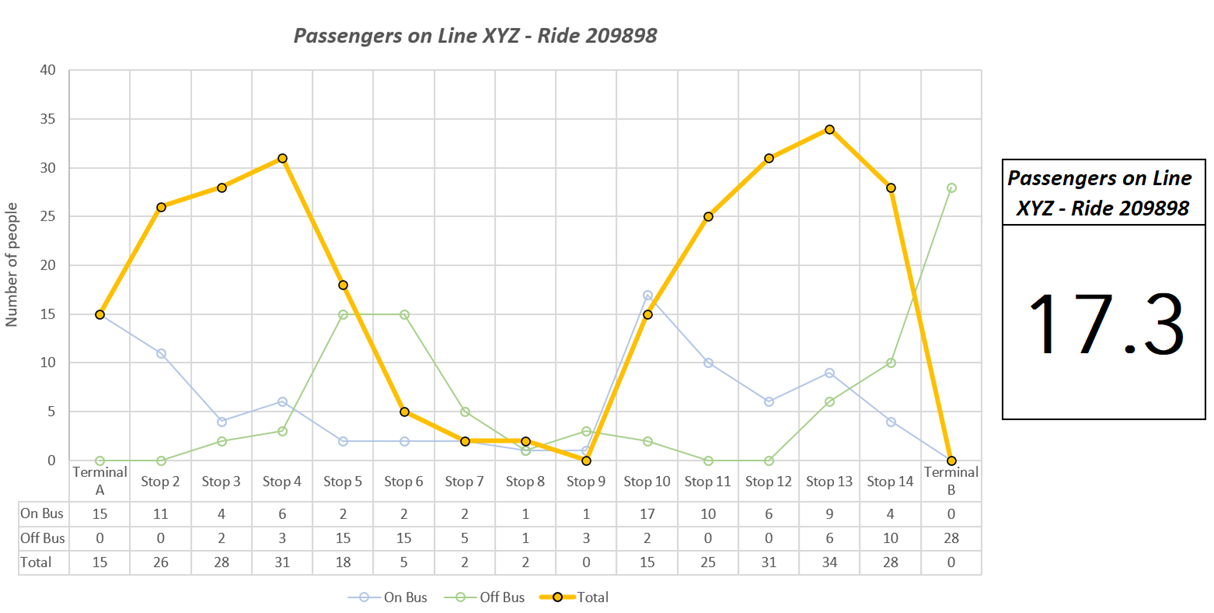
\includegraphics[width=1\textwidth]{Images/New Technologies/dynamic KPIs.png}
    \caption{Dynamic KPIs Example}
    \label{fig:dynKPI}
\end{figure}

\newpage As it is possible to see from the image  \ref{fig:dynKPI}, both are telling the same information, but in two different ways: the number on the right tells us just the mean number of passengers for that particular ride, although looking at the graph on the left we can detect much more information, such as that the central stops of the ride (7, 8 and 9) are very little used, and also the number of passengers on board at that moment are almost none. Here the PTA can make multiple decisions, such as dividing the line into two pieces to maximize the effectiveness of both of them. A deeper analysis can be done to understand why those stops are rarely used, maybe they can be re-positioned to meet higher demand, changing the line route by a little.

\newpage
\subsection{New Technologies KPIs examples}
\label{subsec:newKPIex}
Having know all the knowledge of new technologies that can be installed on and off the buses and all the new process that are involved to built more interesting KPIs, it is time to make some example, directly related to which data has Arriva now and what it could have in the future. In order to maintain the same scheme of pages in the traditional dashboard in \ref{ch:dashboard}, the KPIs are listed in the same structure:
% Please add the following required packages to your document preamble:
% \usepackage{lscape}
\newpage
\thispagestyle{empty}
\begin{landscape}
\begin{table}
\centering
\begin{tabular}{|l|l|l|l|}
\hline
\rowcolor{bluepoli!40}
\multicolumn{1}{|c|}{\textbf{KPI denomination}}                                                    & \multicolumn{1}{c|}{\textbf{\begin{tabular}[c]{@{}c@{}}Technologies \\ Used\end{tabular}}} & \multicolumn{1}{c|}{\textbf{\begin{tabular}[c]{@{}c@{}}Unit of\\  Measure\end{tabular}}} & \multicolumn{1}{c|}{\textbf{Explanation}}                                                                                                                                                        \\ \hline
\begin{tabular}[c]{@{}l@{}}Mean delay by time slot \\ (peak vs. off-peak) and ride\end{tabular}    & AVL, AVM                                                                                   & min                                                                                      & \begin{tabular}[c]{@{}l@{}}Understanding if a  \\delay is mainly caused \\ by the departing hour of the ride, \\ can help to modify   the schedule according to it\end{tabular}                    \\ \hline
\begin{tabular}[c]{@{}l@{}}Visualization on where \\ the ride generates the delay\end{tabular}     & AVL, AVM                                                                                   & map                                                                                      & \begin{tabular}[c]{@{}l@{}}Deepening the   knowledge of the delay \\ can mean even \\better improvements \\ going to make specific   changes \\ in some section of the lines\end{tabular}          \\ \hline
Lost costumers per   suppressed ride                                                               & APC, AVM                                                                                   & \#                                                                                       & \begin{tabular}[c]{@{}l@{}}Knowing how many   \\people are affected \\ by a suppressed ride\\ can help to assess \\ the importance of   that ride and an overall \\ level of discomfort\end{tabular} \\ \hline
Delay amount over mm   of rain                                                                     & AVM, IoT                                                                                   & min/mm                                                                                   & \begin{tabular}[c]{@{}l@{}}Knowing the relation  \\ between delays and \\ weather conditions\\ is important to correctly \\ dimension the   problem\end{tabular}                                     \\ \hline
\begin{tabular}[c]{@{}l@{}}Load Factor per run   \\ per time slot (peak vs. off-peak)\end{tabular} & APC, AVM                                                                                   & \%                                                                                       & \begin{tabular}[c]{@{}l@{}}Knowing the   percentage of load\\  for a particular run can help to allocate \\ better the resources\end{tabular}                                                    \\ \hline
Load Factor vs.   Weather Condition                                                                & APC, IoT                                                                                   & \%                                                                                       & \begin{tabular}[c]{@{}l@{}}Also in this case, knowing \\   the behavior in\\ different weather condition \\ can help to allocate better the resources\end{tabular}                                 \\ \hline
\end{tabular}
\caption{List of new Service Quality KPIs}
\label{tab:servicequality}
\end{table}
\end{landscape}
% Please add the following required packages to your document preamble:
% \usepackage[normalem]{ulem}
% \useunder{\uline}{\ul}{}
% \usepackage{lscape}
\newpage
\thispagestyle{empty}
\begin{landscape}
\begin{table}[]
\centering
\begin{tabular}{|l|l|l|l|}
\hline
\rowcolor{bluepoli!40}
\multicolumn{1}{|c|}{\textbf{KPI denomination}}                                                        & \multicolumn{1}{c|}{\textbf{Technologies Used}} & \multicolumn{1}{c|}{\textbf{Unit of Measure}} & \multicolumn{1}{c|}{\textbf{Explanation}}                                                                                                                                                                                                                             \\ \hline
\begin{tabular}[c]{@{}l@{}}Percentage of low environmental   \\ impact bus on the road\end{tabular}    & AVM                                             & \%                                            & \begin{tabular}[c]{@{}l@{}}Knowing how many green   bus \\ are circulating on the road can be \\ an interesting KPI to show at the PTA\end{tabular}                                                                                                                   \\ \hline
Percentage of km   made by hybrid/EV bus                                                               & AVM, AVL                                        & \%                                            & \begin{tabular}[c]{@{}l@{}}Same as before, knowing  how many kms \\ have been done in a healthy way is useful\end{tabular}                                                                                                                                            \\ \hline
Tons of $CO_2$ emitted   by bus or by line                                                             & AVM                                             & ton                                           & \begin{tabular}[c]{@{}l@{}}Understanding which   model of bus on which line\\  is the most emissive is useful to assess \\ how to renovate   the fleet\end{tabular}                                                                                                   \\ \hline
\begin{tabular}[c]{@{}l@{}}Tons of $CO_2$   \\ emitted in the city center vs. rural areas\end{tabular} & AVM, AVL                                        & ton                                           & \begin{tabular}[c]{@{}l@{}}Knowing the spatial   distribution of tonnage \\ emission can be useful to re-allocate different bus  \\  models on the lines\end{tabular}                                                                                                 \\ \hline
\begin{tabular}[c]{@{}l@{}}Mean bus consumption   \\ per run, per line, per bus type\end{tabular}      & AVL, AVM                                        & $L_{fuel}$/(run,   line, bus)                 & \begin{tabular}[c]{@{}l@{}}Awareness on bus   consumption by run is useful \\ to re-allocate and renovate the rolling stock\end{tabular}                                                                                                                              \\ \hline
Energy consumption curve   for EV bus                                                                  & AVM, AVL                                        & kWh/(time, km)                                & \begin{tabular}[c]{@{}l@{}}Having Electric Vehicle can be difficult to manage \\ in terms of recharging point and time allocation,  \\  understanding where the bus consume most \\ of its energy is handy to optimally   place \\ the recharging points\end{tabular} \\ \hline
\end{tabular}
\caption{List of new KPIs on Rolling Stock}
\label{tab:rollingstock}
\end{table}
\end{landscape}
% Please add the following required packages to your document preamble:
% \usepackage{lscape}
\newpage
\thispagestyle{empty}
% Please add the following required packages to your document preamble:
% \usepackage{lscape}
\begin{landscape}
\begin{table}[]
\centering
\begin{tabular}{|l|l|l|l|}
\hline
\rowcolor{bluepoli!40}
\multicolumn{1}{|c|}{\textbf{KPI denomination}}                                                       & \multicolumn{1}{c|}{\textbf{Technologies Used}} & \multicolumn{1}{c|}{\textbf{Unit of Measure}} & \multicolumn{1}{c|}{\textbf{Explanation}}                                                                                                                                                             \\ \hline
\begin{tabular}[c]{@{}l@{}}Commercial speed \\ deviation   from mean\end{tabular}                     & AVL, AVM, historical   data                     & $\pm$ km/h                                    & \begin{tabular}[c]{@{}l@{}}Comparing real-time   \\ commercial speed with the mean \\ of historical data help understand, \\ together   with delays information, \\ where is the problem\end{tabular} \\ \hline
Amount of km per day                                                                                  & AVM                                             & km                                            & Amount of kilometers   per day                                                                                                                                                                        \\ \hline
Planned vs. Effective   kms                                                                           & AVM                                             & \%                                            & \begin{tabular}[c]{@{}l@{}}Comparison between   \\ planned km on schedule \\ and km effectively done in a day\end{tabular}                                                                            \\ \hline
\begin{tabular}[c]{@{}l@{}}Mean time per stop   \\ (peak vs. off-peak)\end{tabular}                   & AVL                                             & sec                                           & \begin{tabular}[c]{@{}l@{}}Amount of time taken   at each stop to \\ loading and unloading the passengers\end{tabular}                                                                                \\ \hline
\begin{tabular}[c]{@{}l@{}}Stop time in   relation to number \\ of people moved per stop\end{tabular} & AVL, APC                                        & \# of people / sec                            & \begin{tabular}[c]{@{}l@{}}As the one above but    comparing it \\ to the number of people \\ that   actually moved\end{tabular}                                                                      \\ \hline
\begin{tabular}[c]{@{}l@{}}Commercial speed vs.\\ millimeters of rain/snow\end{tabular}               & AVL, IoT                                        & f(Km/h, mm)                                   & \begin{tabular}[c]{@{}l@{}}Comparison between mean  \\  commercial speed \\ of the ride and the amount \\ of rain fall in that period of   time\end{tabular}                                          \\ \hline
\begin{tabular}[c]{@{}l@{}}Commercial speed vs. \\ Fuel Consumption or $CO_2$ produced\end{tabular}   & AVL, AVM                                        & (km/h)/kWh, (km/h)/$tons_{CO\_2}$           & \begin{tabular}[c]{@{}l@{}}Helps understand the   driving behavior \\ of the drivers among with the points \\ where to optimize it\end{tabular}                                                       \\ \hline
\end{tabular}
\caption{List of new Operational KPIs}
\label{tab:operation_indication}
\end{table}
\end{landscape}
% Please add the following required packages to your document preamble:
% \usepackage{lscape}
%\newpage
\thispagestyle{empty}
%\begin{landscape}
\subsection{New Technologies KPIs examples}
\label{subsec:newKPIex}
Having know all the knowledge of new technologies that can be installed on and off the buses and all the new process that are involved to built more interesting KPIs, it is time to make some example, directly related to which data has Arriva now and what it could have in the future. In order to maintain the same scheme of pages in the traditional dashboard in \ref{ch:dashboard}, the KPIs are listed in the same structure:

\begin{table}[H]
\centering
\begin{tabular}{|l|l|l|l|}
\hline
\rowcolor{bluepoli!40}
\multicolumn{1}{|c|}{\textbf{KPI denomination}}                                       & \multicolumn{1}{c|}{\textbf{Technologies Used}} & \multicolumn{1}{c|}{\textbf{UoM}} & \multicolumn{1}{c|}{\textbf{Explanation}}                                                                                                                                                          \\ \hline
\begin{tabular}[c]{@{}l@{}}Daily single tickets   \\ sold over passenger \\ moved\end{tabular}  & Iot, E-Ticketing,   APC                & \begin{tabular}[c]{@{}l@{}} €\\ \ \# people \end{tabular}                                & \begin{tabular}[c]{@{}l@{}}Understand how\\ the amount \\ of single ticket sold affect \\ the overall passenger,\\  helping to size the service   \\ not only on historical \\ data and passes\end{tabular} \\ \hline
\begin{tabular}[c]{@{}l@{}}Distribution of   \\ ticket vs. pass per ride\end{tabular} & E-Ticketing, APC                     & \%                                            & \begin{tabular}[c]{@{}l@{}}Understand which   \\ type of costumer takes \\ certain rides allow to\\  assess decision for a ride\end{tabular}                                                       \\ \hline
\begin{tabular}[c]{@{}l@{}}Annual Fuel cost  \\  over km done\end{tabular}            & AVM, AVL                                        & €/km                                          & \begin{tabular}[c]{@{}l@{}}Helps understand the \\   driving behavior \\of the drivers \\ and the cost percentage \\ that affect \\the   balance sheets\end{tabular}                                   \\ \hline
\end{tabular}
\caption{List of new Economical and Financial KPIs}
\label{tab:economic}
\end{table}
%\end{landscape}

%CAPITOLO SOCIAL SUSTAINABILITY
\section{Social Sustainability}
To define which are the relevant indicators for social sustainability, both in terms of quality of service for customers and as a workplace, it is possible to start from the SDGs listed in the introduction.

\begin{minipage}[c]{0.2\textwidth}
    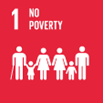
\includegraphics[width=\textwidth]{Images/Social_sustainability/1_no_poverty.png}
\end{minipage}
\begin{minipage}[c]{0.8\textwidth}
    According to the 1.3 SDG to be able to defeat poverty , the salaries must be adjusted to the job position according the national collective labour agreement. To monitor this aspect is useful to consider the following KPI: average salary level in proportion to the national collective labour agreement.
\end{minipage}
\hfill



\begin{minipage}[c]{0.2\textwidth}
    
\includegraphics[width=\textwidth]{Images/Social_sustainability/3_helth.png}
\end{minipage}
\begin{minipage}[c]{0.8\textwidth}
    The 3.6 SDG has the goal to halve the number of deaths and injuries from road traffic accidents worldwide by 2020. To monitor this aspect the following KPIs can be considered:
\begin{itemize}
    \item Number of injuries and deaths caused by road accidents
    \item Number of road accidents
\end{itemize}
\end{minipage}
\hfill

\begin{minipage}[c]{0.2\textwidth}
    
\includegraphics[width=\textwidth]{Images/Social_sustainability/4_education.png}
\end{minipage}
\begin{minipage}[c]{0.8\textwidth}
The 4.4 SDG emphasises the importance of training education in workplace in order to have always better quality of service and to increase safety of workers and clients.
\begin{itemize}
    \item Training hours per capita for traveling and non-traveling personnel
    \item \% Employees who received an evaluation during the year
\end{itemize}
\end{minipage}
\hfill

\begin{minipage}[c]{0.2\textwidth}
    
\includegraphics[width=\textwidth]{Images/Social_sustainability/5_gender.png}
\end{minipage}
\begin{minipage}[c]{0.8\textwidth}
Forms of discrimination and gender disparities are to be considered both transport service customers (5.1 SDG) and company employees (5.5 SDG). Some reference indicators to consider measuring the gender equity are the following:
\begin{itemize}
    \item \% female passengers: this information can be collected easily if the passenger register on the website or on the application of the company 
    \item Number of assaults and violence to women on buses
    \item \% women in management area: more importance on the women full and effective participation and equal leadership opportunities at all levels of decision-making in political, economic and public life
    \item \% women with a permanent contract 
    \item Ratio between training hour for woman and men
\end{itemize}
\end{minipage}
\hfill


\begin{minipage}[c]{0.2\textwidth}
    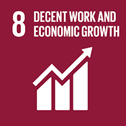
\includegraphics[width=\textwidth]{Images/Social_sustainability/8_work.png}
\end{minipage}
\begin{minipage}[c]{0.8\textwidth}
The 8.2 SDG  stresses the importance to achieve higher levels of economic productivity through diversification, technological updating and innovation, including through a focus on high value-added sectors and labour-intensive sectors. An element to obtain this result is to increase the quality of service.
\end{minipage}
\hfill

Quality of the service has become an element more and more important, for this reason is necessary to define the right KPI to measure the quality of the service and to know how to improve it. The analysis of service quality is of vital importance for both operators and public transport authorities because it plays a key role in attracting new passengers from private cars to the public transport system. The quality of the service depends on many factors; one important factor that become more significant in the last years with the Covid pandemic is the cleaning. The cleaning requirements by the PTA has changed and become stricter.

As reported in the document Carta della mobilità,  the quality of the service can be perceived through a series of fundamental factors that characterize the quality of each aspect of the trip (e.g. travel safety, regularity of the service, cleanliness and hygienic conditions of the vehicles, etc.) and, within each of these, by specific quality indicators (for example for travel safety: number of accidents, age of vehicles) which represent the performance levels of the service provided.

Each factor and quality indicator are associated with a value (which expresses the level of quality of the service actually provided) and a target set each year by the Company providing the service.

The data on customer satisfaction are collected, in accordance with the provisions of the service contracts, with surveys carried out every six months by an external market research company through response surveys. 

More in detail the surveys  analyse the following aspects with their respective KPIs:
\begin{itemize}
    \item Safety of the trip
\begin{itemize}
    \item	Accidents of the vehicles
    \item Passive accidents
    \item Age of vehicles
    \item Total perceived safety of the trip
\end{itemize}
    \item Personal and property safety
    \begin{itemize}
        \item	Complaints (theft and harassment)
        \item Total perceived personal safety
    \end{itemize}
    \item Regularity and punctuality of the service
    \begin{itemize}
        \item 	Regularity of the service
        \item Frequency of rides
        \item Commercial speed
        \item Punctuality in rush hours
        \item Punctuality in non-rush hours
        \item Total perceived regularity of the service
    \end{itemize}
    \item	Comfort and cleanliness of the buses
    \begin{itemize}
        \item Crowding in rush hours 
        \item Crowding in non-rush hours 
        \item Air conditioning
        \item Low-floor bus
        \item Additional services (mobile platform, wheelchair anchoring)
        \item Total perceived comfort
        \item Ordinary cleaning
        \item Extraordinary cleaning
        \item Cleaning of bus stations
        \item Total perceived cleanliness
    \end{itemize}
    \item Information and service to users
    \begin{itemize}
        \item Timeliness
        \item Internal visual devices
        \item Timetable at bus stops
        \item Point of sales of tickets
        \item Feedback to complaints
        \item Total perceived information and services
    \end{itemize}
    \item Relational aspects
        \begin{itemize}
            \item         Total perceived relational aspects
        \end{itemize}
    \item Attention to environment
        \begin{itemize}
            \item Electric or hybrid vehicles 
            \item Use of eco-fuels
            \item Vehicles Euro 3-4
            \item Vehicles Euro 4 and more
            \item Total perceived attention to environment
        \end{itemize}
\end{itemize}

The KPIs are reported in the following figure \ref{fig:kpis}, with a value form 0 (worst situation) to 4 (optimal situation). In 2019 there was an improvement in all indicators, except for the perceived security. For the 2020 the data are not available because the surveys were not carried out due to the Covid pandemic.


\begin{figure}[h]
    \centering
    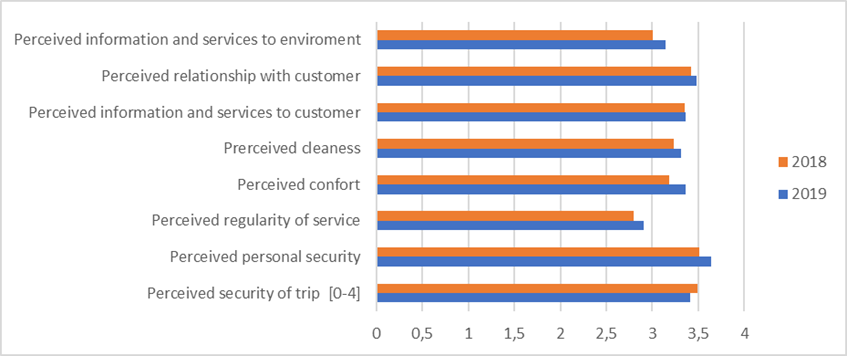
\includegraphics[width=0.9\textwidth]{Images/Social_sustainability/graph.png}
    \caption{KPIs}
    \label{fig:kpis}
\end{figure}
The importance of the cleaning is confirmed in the service contract which establishes penalties in case of:
\begin{itemize}
    \item failure to comply the frequency and/ or cycles in relation to the individual types of intervention (both for ordinary and extraordinary cleaning of the fleet and infrastructure and network systems open to the public).
    \item Insufficient cleaning of the bus (both for ordinary and extraordinary cleaning of the fleet and infrastructure and network systems open to the public).
\end{itemize}
·	


The main requirements for the cleaning are:
\begin{itemize}
    \item	daily cleaning (ordinary cleaning): it consists of removing the filth produced by the passengers, cleaning of cockpit, floor and handrails (about 10-15 min per bus);
    \item monthly cleaning (extraordinary cleaning): it is a deeper cleaning; special products must be used to remove dirt (generally it takes at least 30-40 min per bus)
    \item half yearly cleaning: vehicles are subjected to an antibacterial sanitization and disinfestation cycle 
    \item Nowadays, due to the pandemic situation, the consortium has introduced from March 2020 sanitation interventions with disinfection and sanitization in particular of the surfaces and passenger support points. Also, every fifteen days during the periodic cleaning interventions are performed cleaning by ionization
\end{itemize}


As shown in the results reported in Carta della mobilità, the customer satisfaction surveys (CSS) provide many information on the level of quality of a public transport service.
In addition with the new technologies it is possible to measure:
\begin{itemize}
    \item Regularity and punctuality with AVM
    \item Crowding indicator and possibility of sitting during the journey with passenger counters technology
\end{itemize}

\begin{minipage}[c]{0.2\textwidth}
    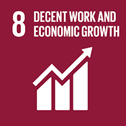
\includegraphics[width=\textwidth]{Images/Social_sustainability/8_work.png}
\end{minipage}
\begin{minipage}[c]{0.8\textwidth}
The 8 SDG remark the importance of an equal and fair salary for all workers, including young people and people with disabilities and the importance to reduce the percentage of unemployed young people who do not follow a course of study or who do not follow training courses. Another aspects is the protection of labour rights and promotion a safe and secure working environment for all workers, including migrant workers, especially migrant women, and those in precarious work. The KPIs useful for this aspect are:
\begin{itemize}
    \item \% employees with permanent contract
    \item \% employees under 35 
    \item \% turnover rate
    \item Frequency of injuries of workers
    \item Index of severity of injuries
    \item Number of hours of training on safety and health
    \item \% employees registered with trade unions
    \item Number of hours of trade union assemblies
    \item Complaints related to work practices
\end{itemize}
\end{minipage}

\begin{minipage}[c]{0.2\textwidth}
    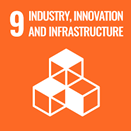
\includegraphics[width=\textwidth]{Images/Social_sustainability/9_industry.png}
\end{minipage}
\begin{minipage}[c]{0.8\textwidth}
The importance of access to information and communication technologies is remarked by the 9.6 SDG. A transport company to achieve that goal could provide a company phone to employees

\begin{itemize}
    \item \% Employees with company phone with application used by the company
\end{itemize}
\end{minipage}

\begin{minipage}[c]{0.2\textwidth}
    
\includegraphics[width=\textwidth]{Images/Social_sustainability/16_peace.png}
\end{minipage}
\begin{minipage}[c]{0.8\textwidth}
The has the goal by 2030, to reduce illicit financing and arms trafficking, enhance the recovery and return of stolen assets and fight all forms of organized crime, reduce corruption and all its forms (16.4), Develop effective, accountable and transparent institutions at all levels (16.6).
To monitor fare evasion, corruption and arms trafficking:
\begin{itemize}
    \item	Number of passengers checked
    \item Number of clients connected on social network
    \item Number of accesses to the site
    \item Courtesy of drivers$\rightarrow$ this information is already collected with the customer satisfaction survey
    \item Number of info point in the area 
    \item Number of point of sales of tickets in the area
\end{itemize}
\end{minipage}
\\
\begin{minipage}[c]{0.2\textwidth}
    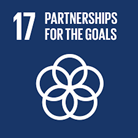
\includegraphics[width=\textwidth]{Images/Social_sustainability/17_partnerships.png}
\end{minipage}
\begin{minipage}[c]{0.8\textwidth}
The 17.13 and 17.17 remind the importance of coordination, coherence to achieve goals global macro-economic stability. 
\begin{itemize}
    \item Number of trade union agreements signed in recent years
    \item Number of partnerships with university
\end{itemize}
\end{minipage}

\section{Green Sustainability}
\label{sec:greensus}
The management of environmental aspects in a public transport company is aimed at their continuous improvement in terms of elimination, reduction or improvement of performance.

For uniform, transparent, goal-oriented and regulation-compliant management, we have to use of a set of procedures built from initial environmental analyses. The main environmental aspects that can be identified among all the material issues are:
\begin{itemize}
    \item Emissions into the atmosphere
    \item Energy Utilization
    \item Water Waste
    \item Waste Production
    \item Use of raw materials and natural resources
    \item Soil Contamination
    \item Dust, odors, vibrations, noise and visual impact problems
\end{itemize}

The significance of impacts can be assessed according to typical environmental analysis criteria, related to the severity, size and frequency of events, taking into account their controllability, applicable legal requirements and the expectations of stakeholders - local communities, employees and public administration. 
The Sustainable Development Goals \ref{sec:Innovative} considered under this aspect are mainly five:
\begin{itemize}
    \item n° 6 – \textit{Clean Water and Sanitation}, for what concerns water waste and overall consumption
    \item n° 7 – \textit{Affordable and Clean Energy}, in particular, considering all the types of energy consumption that a public transport service company have
     \item n° 11 – \textit{Sustainable Cities and Communities}, in particular the 11.6, concerning the emission environmental impact on cities
    \item n° 12 – \textit{Responsible Consumption and Production}, for what concerns raw materials consumption and waste management
    \item n° 13 – \textit{Climate Action}, to combat climate change taking into account all the aspects related to rolling stock, atmospheric and greenhouse emissions
\end{itemize}

\begin{figure}[!ht]
    \centering
    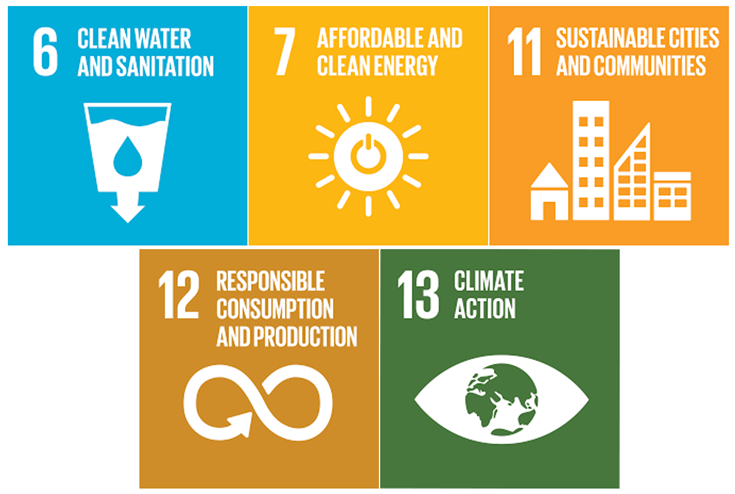
\includegraphics[width=0.6\textwidth]{Images/Green Sustainability/SDGs green.png}
    \caption{Green Sustainability SDGs}
    \label{fig:grsussdg}
\end{figure}

Regarding the five areas of interest in the SDGs \ref{fig:grsussdg}, it can be built a set of KPIs according to the goals previously stated.

\subsection{Energy Consumption}
\label{subsec:enecons}
Referring at the SDG number 7 \ref{tab:onuobjectives}, by 2030 companies have to significantly increase the share of renewable in the global energy mix and double the global rate of energy efficiency improvement.
Energy consumption is mostly derived from bus fuels, which can be reduced through fleet renewal, maintenance activities and improved driving style. In addition to the consumption of buses, other sources of consumption have to be monitored, such as the electricity, natural gas and heating oil at the operational sites.
Looking at the overall activities that a company can perform, here in the table \ref{tab:sourceconsump} are listed some of the main sources of consumption:
\begin{table}[h!]
\centering
\begin{tabular}{l|l|}
\cline{2-2}
                                            & \cellcolor{bluepoli!40}Consumption   of:                                                                                 \\ \hline
\multicolumn{1}{|l|}{Running Buses}         & \begin{tabular}[c]{@{}l@{}}Fuel (diesel and natural gas)\\ Urea (Ad Blue)\\ Antifreeze\\ Lubricants\\ Tyres\end{tabular} \\ \hline
\multicolumn{1}{|l|}{Bus Maintenance}       & \begin{tabular}[c]{@{}l@{}}Spare parts\\ Electrical energy\end{tabular}                                                  \\ \hline
\multicolumn{1}{|l|}{Vehicle Cleaning}      & \begin{tabular}[c]{@{}l@{}}Water resources\\ Electrical energy\\ Detergent consumption\end{tabular}                      \\ \hline
\multicolumn{1}{|l|}{Refuelling}            & Electrical energy                                                                                                        \\ \hline
\multicolumn{1}{|l|}{Vehicle Storage}       & \begin{tabular}[c]{@{}l@{}}Soil\\ Electrical energy\end{tabular}                                                         \\ \hline
\multicolumn{1}{|l|}{Administration}        & \begin{tabular}[c]{@{}l@{}}Methane\\ Soil   \\ Electrical energy\\ Office supplies\end{tabular}                          \\ \hline
\multicolumn{1}{|l|}{\begin{tabular}[c]{@{}l@{}}Supply of goods, \\ materials and services\end{tabular}} & Fuel, Electrical energy, Office supplies                                                               \\ \hline
\end{tabular}
\caption{Main Sources of Consumption for a LPT company}
\label{tab:sourceconsumption}
\end{table}

With that in mind we can identify a set of indicators that can help monitor all of those aspects:
\begin{itemize}
    \item Gasoline and Methane consumption in GJ per km traveled by year
    \item Electrical Energy share usage with respect to previous years
    \item Green Energy used in each activity share
    \item Electricity Consumption share for electricity and heating of offices and sites compared to total energy consumption
    \item Green or Renewable fuel share over the totality of fuel used
    \item Energy Consumption share in relation to every km traveled with respect to the previous year
\end{itemize}

\subsection{Atmosphere and GHG Emissions}
\label{subsec:ghgemissions}
Between 1990 and 2018, emissions of all greenhouse gases in Italy decreased from 516 to 428 million tonnes of CO2 equivalent, a change achieved mainly by reducing carbon dioxide emissions, which contribute 81.4 \% of the total. Emissions in 2015 were 17.1\% lower than in 1990.

\begin{figure}[h!]
    \centering
    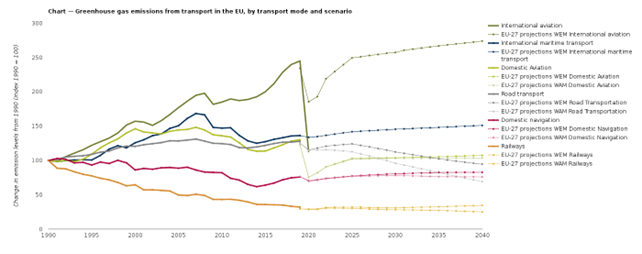
\includegraphics[width=1\textwidth]{Images/Green Sustainability/GHG emission.png}
    \caption{Greenhouse gas emissions from transport in the EU, by transport mode and scenario \cite{GreenhouseScenario}}
    \label{fig:ghgemissions}
\end{figure}

The energy production and transport sectors are the most important, contributing half of the national climate gas emissions. Compared to 1990, however, GHG emissions from the transport sector show a slight increase (3.2\%), while emissions from energy production and industrial installations are clearly decreasing (-23.7\% and -38.9\% respectively).

In this scenario, sustainable mobility is destined to play an important role since the increase in Local Public Transport can make a significant contribution to reducing emissions: Arriva therefore has to contribute to the transition to more energy and emission-efficient transport.
There are some actions that the company can undertake in order to commit gradually to this cause, such as:
\begin{itemize}
    \item Identify the activities that produce direct and indirect emissions both at atmospheric level and at greenhouse level
    \item Monitor and analysis of the emissions produced
    \item Implement projects and actions aimed at reducing them as well as measuring their effectiveness
    \item Raise internal and external awareness of this issue through reporting and communication to the stakeholders.
\end{itemize}

Greenhouse gas emissions can be reported in accordance with the GHG protocol (Greenhouse Gas protocol) \cite{ghgprotocol} which provides for the distinction into three categories:
\begin{description}
   \item[Scope 1] Direct emissions from the combustion of fossil fuels (diesel and natural gas) for road transport - bus fleet and car fleet - for the production of thermal energy and emissions of refrigerant gases from air conditioning systems. 
   \item[Scope 2] Emissions resulting from the production of electricity taken from the grid and consumed for the operation of plants and for lighting; the company is indirectly responsible for the emissions generated by the energy supplier for the production of the energy required. 
   \item[Scope 3] Indirect emissions, other than those from electricity consumption, which are a consequence of the company's activities and which arise from sources not owned or controlled by other organizations. The boundary of Scope 3 is defined by the organization and generally includes what can be quantified and influenced by the company.
\end{description}

As a partial solution for direct atmosphere emissions from the rolling stock, vehicles can be equipped with the innovative SCR - Selective Catalytic Reduction - system, which uses urea-based liquid, to reduce exhaust emissions in terms of particulate matter and nitrogen oxides. The system is able to reduce harmful substances in the exhaust gas of diesel vehicles by up to 80 per cent.

Wanting to quantify all of that, here below are listed some example KPIs:
\begin{itemize}
    \item Emissions of greenhouse gases (CO2, CFCs, CH4, etc.) per passenger transported or per km travelled
    \item Generic emissions (PM, VOCs, NOx, CO, etc.) per passenger transported or per km travelled
    \item Air quality standards and management plans. 
    \item Rolling Stock share with Euro5, Euro6 or EEV motorization
    \item Total km travelled by low-impact buses share
\end{itemize}

\subsection{Water Discharges and Waste Management}
\label{subsec:water}
The production of waste mainly originates from maintenance activities and bus washing. Improve the quality of water discharges from washing vehicles that may contain pollutants, such as hydrocarbons, oils and various powders is a main component of the green approach of a company Along with adequate purification plants regular inspections of the plants should be carried out, directly by the company. In the event of an emergency situation, all activities that produce water to be purified destined for the plant concerned should be suspended until the plant is operational again.

Purifiers and absorbent material will produce sludge, extracted during inspections and maintenance, which have to be stored in the plants themselves or in labeled containers at each site. The frequency of interventions has to be established on the basis of the indications in the maintenance booklets and those provided by the installer, as well as the actual use of the systems.

Storm water runoff from forecourt areas should be conveyed to plants for treatment, as required by regulations. To avoid possible contamination of runoff water the PTO can take some precautionary measures, such as:
\begin{itemize}
    \item Workshop activities have to take place in covered areas without sumps
    \item Waste storage have to takes place in covered areas and containers
    \item Storage areas that could give rise to environmental impacts on water discharges must be included in a water discharge monitoring plan
    \item Sumps and collection tanks must be inspected periodically and cleaned at least once a year
 \end{itemize}

According to all the procedures listed above, we have selected a list of KPIs that could be useful to track down this particular topic inside the company:

\begin{itemize}
    \item Liters shares of reused water
    \item Liters of storm water saved per year
    \item Tons of waste generated per year
    \item Mean time to inspection on service hours
    \item Percentage of hazardous waste recovered
    \item Tons of waste produced per 1000km traveled
\end{itemize}


%capitolo seyed


